\section{Prozessverwaltung}
\label{chapProcess}
Das Betriebssystem weist die Eigenschaften eines präemptiven Multi-Tasking-Systems, mit \textit{Round-Robin}-Verfahren und fixer Zeitscheibe, auf. Für die Verwaltung der einzelnen Prozesse und den Wechsel des aktiven Prozesses, wurde eine Prozessverwaltung implementiert. Im Folgenden sind die beteiligten Komponenten und wichtigen Eigenschaften der Prozessverwaltung dokumentiert.

\subsection{Prozesszustände}
Jeder Prozess besitzt zu jedem beliebigen Zeitpunkt einen fix definierten Zustand, welche ebenfalls fix definierte Zustandsübergänge aufweisen, d.h. es können keine Inkonsistenzen diesbezüglich auftreten. Abbildung \ref{fig:Process-states} zeigt die verschiedenen Zustände eines Prozesses sowie die jeweilig erlaubten Übergänge zu einem anderen Zustand auf.

\begin{figure}[H]
	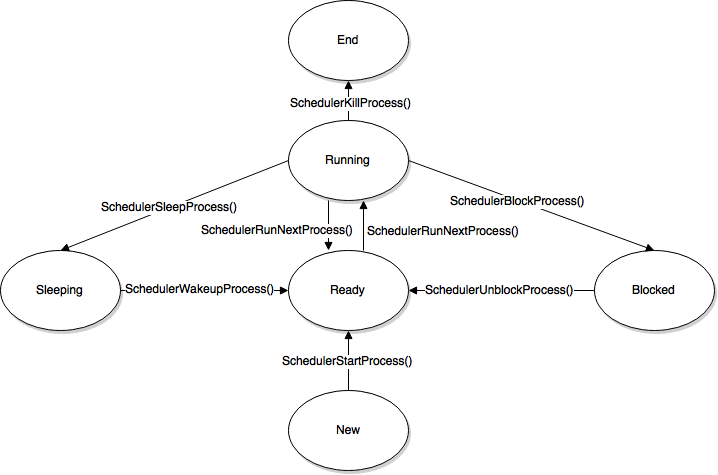
\includegraphics[scale=0.60]{chapters/processmanagement/figures/StateTransition}
	\caption{Prozesszustände und Zustandsübergänge}
	\label{fig:Process-states}
\end{figure}

Im folgenden wird eine detaillierte Erklärung zu den einzelnen Zuständen aus Abbildung \ref{fig:Process-states} gegeben.

\begin{description}
	\item[\textit{Ready}] \hfill \\
	Der Zustand \textit{Ready} tritt ein, wenn ein Prozess zur Ausführung bereit ist. Neu erstellte Prozesse befinden sich in jedem Fall im Zustand \textit{Ready}.
	
	\item[\textit{Running}] \hfill \\
	Ein Prozess weist diesen Zustand auf, wenn er sich in Ausführung befindet, respektive der Prozessselbst die aktuelle Zeitscheibe in Anspruch nimmt.
	
	\item[\textit{Blocked}] \hfill \\
	Ein Prozess weist den Zustand \textit{Blocked} auf, wenn dieser von der Ausführung durch ein bestimmtes Ereignis abgehalten wird, beispielsweise wartet der blockierte Prozess auf das Beenden eines anderen Prozesses.
	
	\item[\textit{Sleeping}] \hfill \\
	Falls ein Prozess für eine gewisse Zeit keine Prozessorzeit benötigt, kann er sich selbst über die System-API in den Zustand \textit{Sleeping} versetzen.

\end{description}

\subsection{Scheduler}
\label{secScheduler}
Der \textit{Scheduler} ist eine Kernelkomponente welcher die Prozesse aus einer abstrakten Sicht, respektive lediglich die Prozesszustände und deren Kontext, verwaltet. Die Schnittstelle des \textit{Scheduler} ist in Listing \ref{lstScheduler} angeführt.

\lstinputlisting[language=C, caption=Implementierung der DriverManager Schnittstelle für den LED Treiber, captionpos=b, label=lstScheduler]{chapters/processmanagement/codefiles/scheduler.c}

Die \textit{Scheduler}-Funktion \texttt{SchedulerRunNextProcess(..)} kann zu jedem beliebigen Zeitpunkt aufgerufen werden, an dem der aktuelle \texttt{context\_t} vorhanden ist, vorwiegend wird diese Funktion aber vom Timer-\textit{Interrupt} aufgerufen, welcher die Zeitscheibe von $10ms$ realisiert.\\
Die Zeitscheibe von $10ms$ wurde auf Basis verschiedener Experimente gewählt und hat sich, aufgrund dessen dass keine Priorisierung der Prozesse erfolgt, als annehmbar herausgestellt. Die durchgeführten Experimente in Kapitel \ref{Performanz} haben aber gezeigt, dass möglicherweise eine längere Zeitscheibe zu einer besseren Gesamtperformanz geführt hätten.

\subsection{ProcessManager}
\label{secProcessManager}
Der \textit{ProcessManager} ist eine dem \textit{Scheduler} übergeordnete Komponente, welche eine weitere Verwaltung der Prozesse realisiert. Der \textit{ProcessManager} fügt den abstrakten Eigenschaften der Prozesse des \textit{Schedulers} zusätzlich noch Meta-Informationen, wie Prozessname, Startzeit usw. hinzu. Der \textit{ProcessManager} stellt dabei die Schnittstelle für andere Kernelkomponenten zur Verfügung um Prozesse zu starten und zu beenden.\\

Das Vorgehen bei der Prozessverwaltung wird im Sequenzdiagramm von Figure \ref{Sequencediagram} dargestellt. Ein Client übergibt dem \textit{ProcessManager} die Aufgabe einen Prozess zu erzeugen. Dieser delegiert das Erzeugen des Prozesses an den Scheduler weiter. Hierbei ist zu beachten, dass die Meta-Informationen vom \textit{ProcessManager} nicht weitergegeben werden. Der Scheduler speichert sich diesen neuen Prozess in seiner Prozesstabelle ab. Der \textit{MemoryManager} allokiert nun den vom Prozess benötigtem Speicherplatz. Der erzeugte Prozess wird an den \textit{ProcessManager} zurückgegeben. Dem Client wird nun der Erfolg der Prozesserstellung mitgeteilt, respektive wird diesem die erzeute Prozess-ID zurück geliefert.

\begin{figure}[H]
	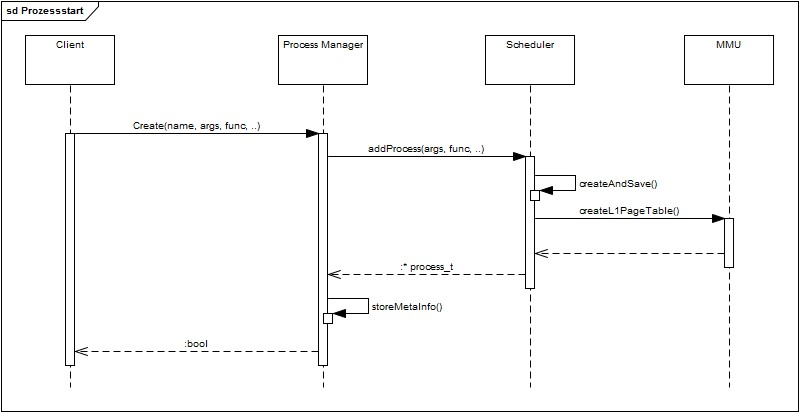
\includegraphics[scale=0.70]{chapters/processmanagement/figures/processmanagement-sequence-diagram}
	\caption{Sequenzdiagramm der Prozessverwaltung}
	\label{fig:Sequencediagram}
\end{figure}

\pagebreak 